\section{Experiment}
In the reproducibility experiments, we re-implement FixMatch from scratch using PyTorch and reproduce the essential experiments in the original paper with the similar results.
We use the hyperparameters 
($\lambda_u = 1,\, \eta = 0.03,\, \beta=0.9,\, \tau=0.95,\, \mu = 7,\, B = 64,\, K = 2^{20}$) 
given by \citep{sohn2020fixmatch} and focus on reproducing the performance on CIFAR-10 (Sec. 4.1 of \citep{sohn2020fixmatch}) and barely supervised learning experiments (Sec. 4.4 of \citep{sohn2020fixmatch}). Besides the early introduced hyper-parameters, we use SGD with $\beta = 0.9$ for training the model, and the learning rate is decay with $\eta \cos (\frac{7\pi k}{16 K})$, where $K$ is the total time step and $k$ is the current time step. Each experiment takes around 68 hours on a single V100. And all the error rates is generated from EMA (exponential moving average) of models in the SGD training trajectory.

% Instead of using computational resources for hyperparameter tuning and ablation study (Sec. 5 of \citep{sohn2020fixmatch}), 
% \RT{What we did for reroducibility. A high level description.} 

% the performance of it by replicating similar results shown in the second-last row of Table 2 under section CIFAR-10 in the paper.
Then, we investigate  confirmation errors of "Match"-based SSL methods to see whether there exists such error and asymmetric noise of pseudo labels in FixMatch with the official experiment setup, i.e. unbalanced batches, in  \citep{sohn2020fixmatch}.
Next, we examine the existence of confirmation errors and asymmetric noise for FixMatch again in a more reliable way using re-constructed batches as introduced in Sec. \ref{sec:method}. 
Furthermore, we respectively add the equal-frequency entropy regularization and confidence entropy regularization on the labeled training data in the loss function and compare with the baseline FixMatch without entropy regularization on the BC batches. Finally, we add asymmetric noise to the labeled data in the training dataset and compare the performance of baseline FixMatch and FixMatch with different entropy regularization.

\subsection{Reproducibility} \label{sec:rep}
\paragraph{CIFAR-10.}
We reproduced the experiments on CIFAR-10 with 40, 250, 4000 labeled data and 5000 validation samples as the official implementation of FixMatch\footnote{The official implementation: \url{https://github.com/google-research/fixmatch}. From the reproducibility and readability, the official code is not a valid submission.}.  But due to the limitation of computational resources, we didn't reproduce 5 "folds". Thus, our result based on 1 fold doesn't have the standard deviation. Our model uses the Wide ResNet-28-2 \citep{zagoruyko2016wide} with leaky ReLU activation function. 
Our results are shown in Table \ref{tab:err} which is comparable to the performance in \citep{sohn2020fixmatch}.
% in the sense of lack of computational resources. 
% Note that we didn't run over all the training step and only have $105$ epochs out of total 1024 epochs.  
% \citet{sohn2020fixmatch} claim that FixMatch is the one of few works evaluated on less than 400 labeled training data. 
% Our implementation has reasonably good performance on the dataset with 250 labeled data, however, it has poor performance in the dataset with 40 labeled data. 
% Therefore, our implementation has reasonable results when there are not too few labeled data in training dataset. We further explore the required minimum number of labeled data for our implementation. We found that $20.79\%$ error rate with 100 labeled data in training dataset and $11.5\%$ error rate with 150 labeled data in the training dataset. Therefore, the minimum number of required labeled data in the training dataset can be around 100 ($40 < 100 < 150$) considering the error rate pattern in Table \ref{tab:err}.

\begin{table}[h]
\centering
\small
\caption{ Error rates for CIFAR-10 on test data. FixMatch (RA) uses RandAugment \citep{cubuk2020randaugment}. BC means that the experiment uses balanced-class batches as introduced in Sec. \ref{sec:method}. We use the experiment with BC and RA as a comparison baseline results for the investigation in Sec. \ref{sec:exp_noise}. 
% \lc{It also shows that the performance of our implementation with and without BC batches are barely distinguishable.(we don't have results with BC batches)}
} \label{tab:err}
\begin{tabular}{cccccc}
\hline
              & \multicolumn{3}{c}{CIFAR-10} \\ \hline
Method        & 40 labels     & 250 labels     & 4000 labels     \\ \hline
Official FixMatch (RA) & $13.81 \pm 3.37$      & $5.07\pm 0.65$        &     $4.26\pm 0.05$     \\ 
Ours (RA) & $10.04$     & $5.29$        &     $4.36$     \\ 
% Ours (RA+BC) & $39.85 \sim 40.10$   & $10.84 \sim 11.07$        &     $6.33 \sim 6.57$    \\ 
\hline
\end{tabular}
\end{table}

\paragraph{Barely supervised learning.}
We also reproduce the one example per class experiment.
\citep{sohn2020fixmatch} hypothesize that the repressiveness of the chosen labeled data influences the results significantly. Since there are only one/few samples per class, this hypothesis is reasonable intuitively. Then, \citet{sohn2020fixmatch} categorized the training dataset into eight levels of “prototypicality”, i.e., representative of the underlying class and then ordered the training samples by their “prototypicality”. With the same hyperparameters, the model is trained with $10$ provided most representative labeled data under Random Augment. The accuracy is $84.41\%$ compared with the official implementation: a median of $78\%$ accuracy and a maximum of $84\%$ accuracy. 
% Since the minimum number 100 of labeled data for our implementation is larger than the one 40 of the official implementation, we hypothesize that for the barely supervised learning experiment we also need more labeled data than 10. Unfortunately, we didn't have more time to spend on choosing more representative labels for the experiment and more computational resources for this specific experiment.

\subsection{Ablation studies}
The ablation studies are based on FixMatch with 250 labels using CTAugment. 
\paragraph{Study for Confidence threshold.}
We performance the ablation studies for confidence threshold. Due to the limited computation resource, we hypothesize that experiments with lower confidence threshold will achieve worse performance and explore more values around the optimal value of confidence threshold, 0.95 chosen by the authors. Thus our examined threshold value is between 0.7 to 0.98. As shown in Figure\ref{fig:abastudy} (c), the error rate is between $6.54\%$ and $6.19\%$ and the highest performance is under the threshold 0.98.  

\begin{figure}[h]
\centering
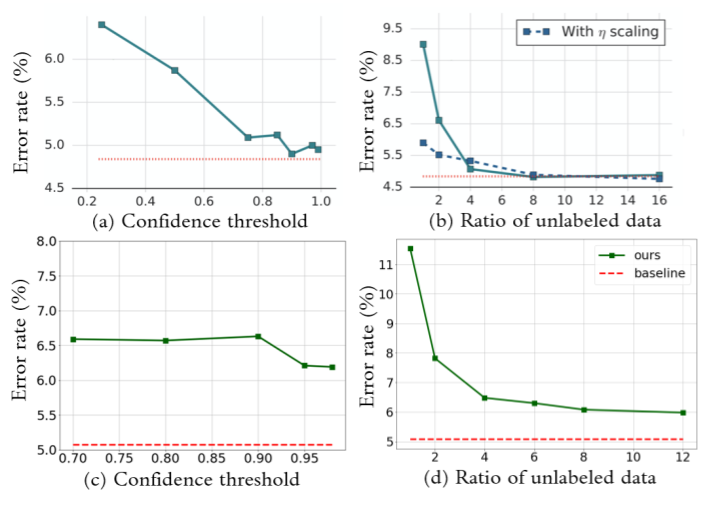
\includegraphics[width=14cm]{../openreview/fig/FixMatch.png}
\caption{Plots of various ablation studies on FixMatch compared with those reported in the paper. (a) Varying the confidence threshold for pseudo-labels in the original paper. (b) Varying the ratio of unlabled data ($\mu$) in the original paper. (c)Varying the confidence threshold for pseudo-labels based on our implementation. (d) Varying the ratio of unlabled data ($\mu$) based on our implementation.
}\label{fig:abastudy}
\end{figure}



\paragraph{Ratio of unlabeled data.}

We perform FixMatch under different ratios of unlabeled data. Figure\ref{fig:abastudy} (d) shows the error rate which is decreasing when the ratio of unlabeled data is higher. A significant increase of the accuracy happens using a large number of unlabeled data. The results show the consistency with the finding in the original paper.

% \begin{figure}[h]
% \centering
% 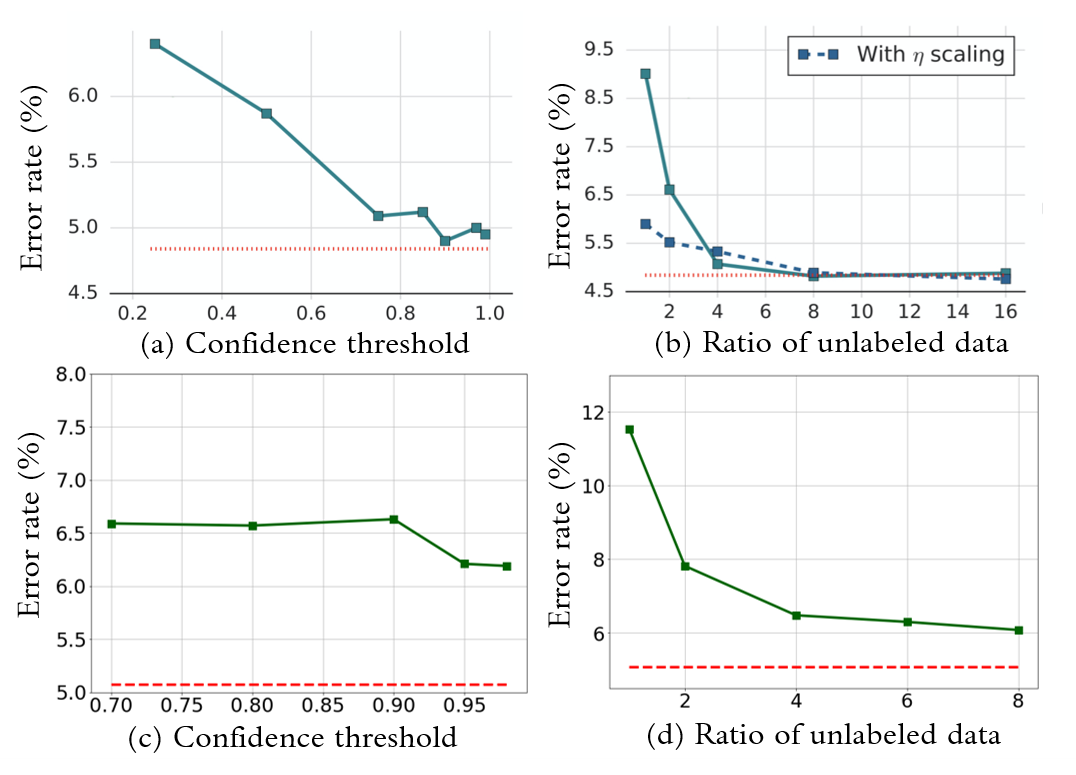
\includegraphics[width=14cm]{fig/ablation.png}
% \caption{
% }\label{fig:abastudy}
% \end{figure}


\subsection{Investigation on confirmation errors and asymmetric noisy (pseudo) labels} \label{sec:exp_noise}
In this section, we show the investigation on confirmation errors and asymmetric noise in labels and pseudo labels and whether the entropy regularization in loss functions \eqref{eq:eqr} and \eqref{eq:cer} can deal with them and improve the performance of FixMatch. The training dataset contains 150 labeled data before augmentation and each BC batch in the training phase contains images with uniformly distributed classes.

\paragraph{Existence of asymmetric noise and confirmation errors in pseudo labels.} We examine the existence of asymmetric noise in pseudo labels by checking the confusion matrix of the prediction of unlabeled data in different batches. Top figures of Figure \ref{fig:cfmx} show the confusion matrices in the experiments without using BC batches. We find that asymmetric noise appears in a random manner, which is as our expectation as analyzed in Sec. \ref{sec:method}. The stochastic behavior is inherited from the randomness of batch composition. Next, we evaluate the asymmetric noise with BC batches, which is a more reliable way as mentioned in Sec. \ref{sec:method}. We found that there exists consistent asymmetric noise, which leads to the confirmation errors, i.e., the model always tends to wrongly predict certain images into certain classes as shown in bottom figures of Figure \ref{fig:cfmx}.
Moreover, the accuracy of our implementation is $93.6\%$ without BC batches and $93.8\%$ with BC batches, which shows that using BC batches has rarely influence on the model performance compared with the one without BC batches.

\begin{figure}[h]
\centering
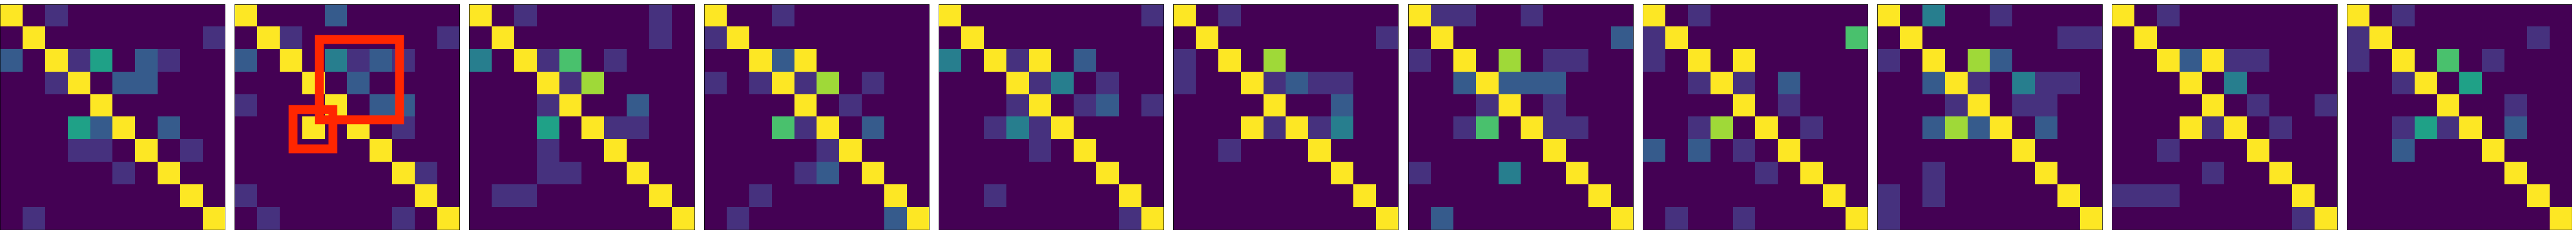
\includegraphics[width=14cm]{../openreview/fig/uBC.png}\\
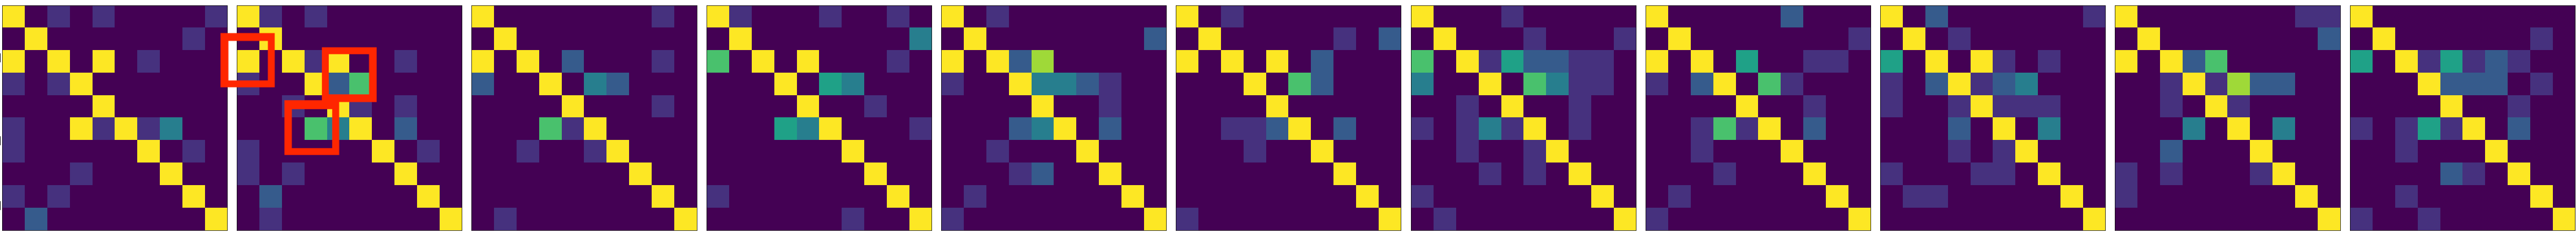
\includegraphics[width=14cm]{../openreview/fig/BC.png}
\caption{Confusion matrices of the confident prediction on unlabeled data with different batch structures.
Confusion matrices are plotted every 100 training steps in the 1st epoch (1024 steps).
The \textbf{top} matrices are from the experiments without BC, and the \textbf{bottom} matrices are the ones with BC. The red areas represent the asymmetric noise in the pseudo labels. The bottom matrices have a stable and smooth transition while the top matrices have a fluctuating transition in the red areas. The yellow color represents larger value and the darker green color represents smaller values.
}\label{fig:cfmx}
\end{figure}

\paragraph{Equal-frequency and confidence entropy regularization on the labeled data.}
Due to limitation of the computational resources, we didn't explicitly run grid search for the hyperparameters in the Equal-Frequency (EF) loss function  \eqref{eq:eqr} and Confidence-Entropy (CE) loss function \eqref{eq:cer}. Instead, we found that for the baseline method the training loss is around 0.2. We then compute the equal-frequency entropy loss for the ideal scenario, equal frequency for all classes, which is $ 0.1 \times \ln 0.1 \approx 2 $. We decide to try the hyperparameter $\lambda_{ce}$, $\lambda_{ef}\leq 0.1$ to avoid making the entropy regularization loss dominate the loss value. Then, we do a hyper-parameter search for the loss function \eqref{eq:eqr} and \eqref{eq:cer}. For all experiments in this experiment, we used cosine function decay for the parameters $\lambda_{ce}$ and $\lambda_{eq}$, which starts with value $1$ and ends with value $0$ in the training phase. We find that using the loss function \eqref{eq:cer} can achieve a better accuracy performance $94.01\%$. Moreover, as an advantage, using the confidence entropy regularization can reduce the asymmetric noise as shown in the bottom confusion matrices of Figure \ref{fig:cfmx_eta}. 
As for the equal-frequency entropy regularization, it has a better accuracy, $93.85\%$. Moreover, the equal-frequency entropy regularization can penalize the asymmetric noise, which may transform it into symmetric noise as shown in the middle confusion matrices of Figure \ref{fig:cfmx_eta}. Note that there are plenty of ways to deal with symmetric noise, which is much easier to handle.

\begin{table}[!h]
\centering
\caption{Error rates on testing data using the loss function \eqref{eq:eqr} and \eqref{eq:cer}. The experiments use 150 labeled data and CTA for training. The first column is the results without BC batch and the second column is the baseline result without using EF or CE regularization.}\label{tab:hp_e}
\begin{tabular}{ccccc}
\hline
Entropy regularization & noBC+Null & BC+Null   & BC+CE    & BC+EF \\ \hline
$\lambda_{ce}/\lambda_{ef}$ & 0  &0  &    0.1 & 0.1 \\ \hline
Error rate    & 6.4 &6.2&    \textbf{5.99}    & 6.15 \\ \hline
\end{tabular}
\end{table}

\begin{figure}[h]
\centering
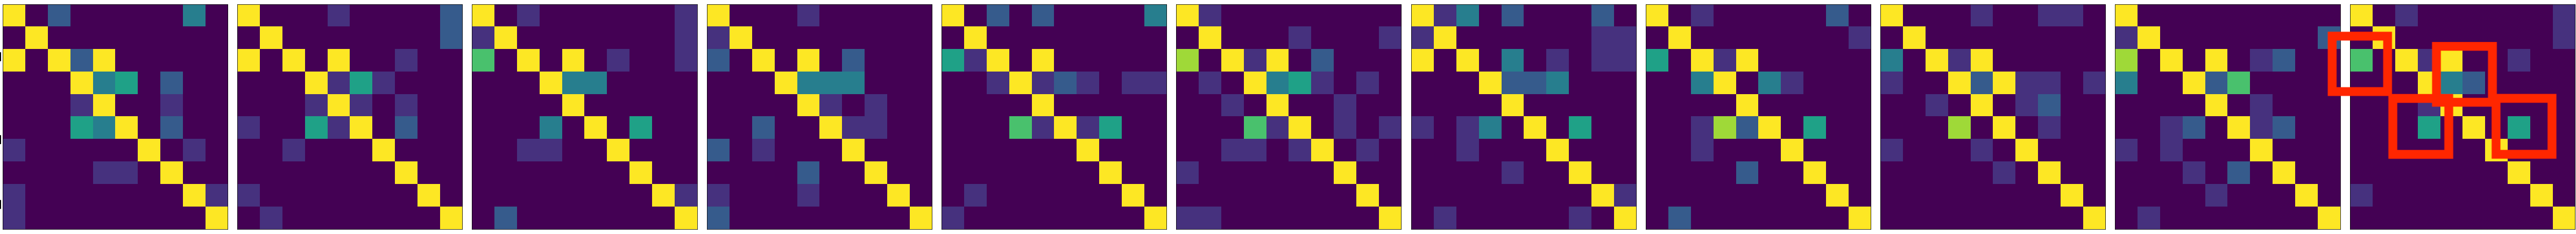
\includegraphics[width=14cm]{../openreview/fig/eta0.png}\\
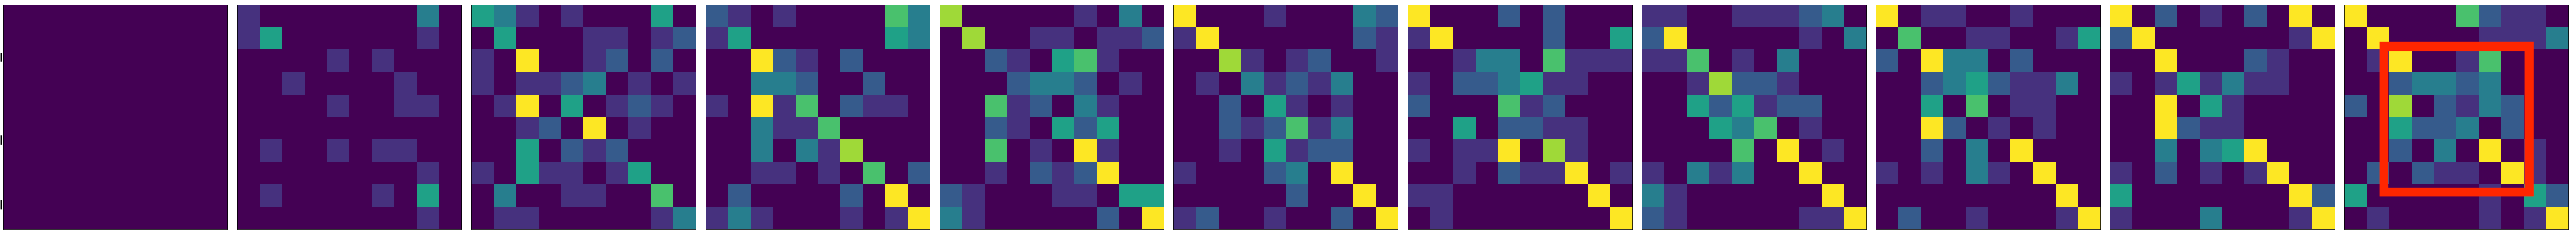
\includegraphics[width=14cm]{../openreview/fig/2eta005.png}\\
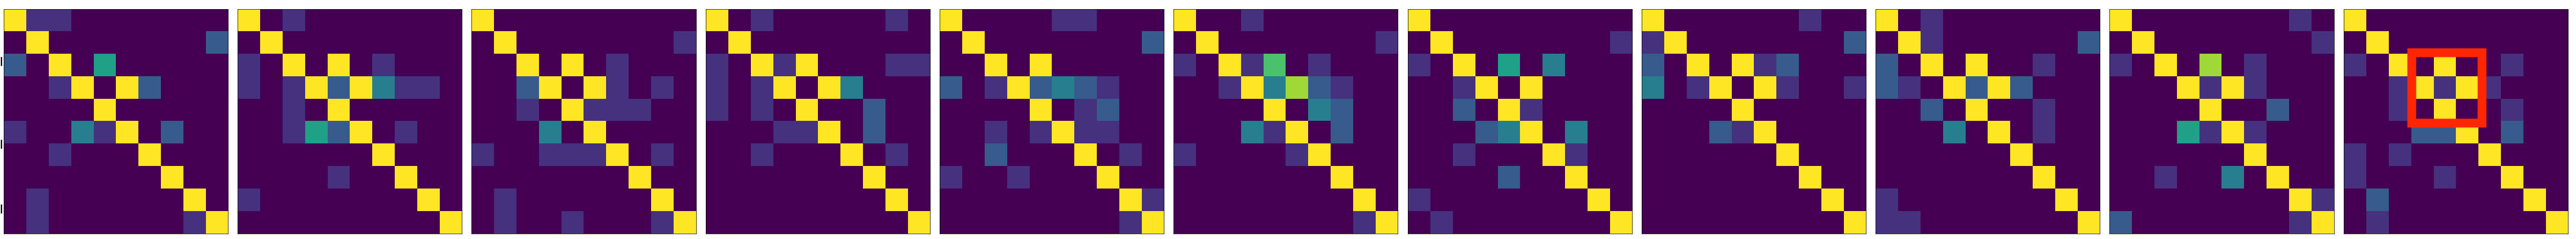
\includegraphics[width=14cm]{../openreview/fig/eta005.png}
\caption{Confusion matrices of the confident prediction on unlabeled data with BC batches using loss functions \eqref{eq:bsl} without entropy regularization at \textbf{top}, 
\eqref{eq:eqr} with equal-frequencey entropy regularization in the \textbf{middle},
and \eqref{eq:cer} with confidence entropy regularization at \textbf{bottom}. Confusion matrices are plotted every 100 training steps in the 1st epoch (1024 steps). The red areas represent the asymmetric/symmetric noise in the pseudo labels. The yellow color represents larger value and the darker green color represents smaller values.
}\label{fig:cfmx_eta}
\end{figure}

\paragraph{Equal-frequency and confidence entropy regularization on the labeled data containing asymmetric noise.}
In this experiment, we use RA data augmentation and manually add asymmetric noise to the labeled data in the training dataset to compare how FixMatch with different loss functions performs in the presence of asymmetric noise in the labeled data.
We respectively select $3$ images from class $0$ and class $1$ in the validation dataset. Then, for the labeled data in the training dataset, we keep the labels unchanged and replace $3$ images in class $2$ with the $3$ images in class $0$. Similarly we replace $3$ images in class $3$ with the $3$ images in class $1$. In this way, the only difference with the previous experiments in this section is that our final validation dataset has $4994$ images and the labeled data in the training dataset contain asymmetric noise. 
Table \ref{tab:ans} shows error rates on 6 runs with different random seeds.
In the presence of asymmetric noise in labeled training data, all proposed methods perform better than the baseline method, in which FixMatch with BC batches decreases the average error rate from 8.6 to 7.37, and the combination of confidence-entropy regularization and BC batches further lowers the error rate to 6.98.
\begin{table}[!h]
\centering
\caption{Error rates of FixMatch methods in the presence of asymmetric noise in labeled training data augmented by RA: 
The baseline method ($\lambda=0$);
The method ($\lambda=0$) with BC batches;
the method with confidence-entropy regularization ($\lambda_{ce}=0.1$) and BC batches;
the method with equal-frequency regularization ($\lambda_{ef}=0.1$) and BC batches.
% The second column is the accuracy of the baseline FixMatch, the third column is the accuracy of FixMactch using equal-frequency regularization, and the last one is the accuracy of FixMatch using confidence entropy regularization after 60 epochs.
}\label{tab:ans}
\begin{tabular}{cccc|c}
\hline
          & $\lambda=0$(noBC) & $\lambda=0$(BC)   & $\lambda_{ef}=0.1$(BC)   & $\lambda_{ce}=0.1$(BC)\\ \hline
Error rates on test data   & $8.6 \pm 2.81$ & $7.37 \pm 2.05$ & $7.95 \pm 2.2$  & \textbf{6.98 $\pm$ 1.83} \\ \hline
\end{tabular}
\end{table}

% 4) we only use the noise-robust loss function for pseudo labels of unlabeled data without balanced-class batches. Only for the pseudo labels because we believe the data in CIFAR-10 do not have noisy labels. 
% \RT{We also need to the hyper-parameter tuning for the loss function in Eqn. \eqref{eq:nrloss}.}

